\documentclass[a4paper,11pt,oneside,openany]{jsbook}
\usepackage{myjlabthesisstyle}
\daigaku{青山学院大学}
\gakubu{社会情報}
\gakka{社会情報学科}
\syubetsu{卒業論文}
\labname{宮治研究室}
\chiefexaminer{宮治~~裕~~教授}

%%%%%%%%%%%%%%%%%%%%%%%%%%%%%%%%%%%%%%%
% ここから先「ここまで個人設定」の範囲に
% 各自の固有の情報を記入して下さい
%%%%%%%%%%%%%%%%%%%%%%%%%%%%%%%%%%%%%%%
\nendo{2024年度}
\teisyutsu{2024年~~1月}
\snum{38122001}
\jname{黒川~~皇輝}
\thesistitle{訪日観光客を対象とした風水害注意情報提供システム} %タイトルを記入
%\thesissubtitle{\LaTeX の利用} %サブタイトルを記入 ない場合はコメントアウト
%\SUBTtrue %サブタイトル有りの場合 ない場合は,コメントアウト
\SUBTfalse %サブタイトル無しの場合 有る場合は,コメントアウト
%%%%%%%%%% ここまで個人設定 %%%%%%%%%%%%%%

\begin{document}

\chapter{はじめに}
本論文では,気象庁が発表する早期注意情報を利用し,訪日観光客が風水害の影響を受ける前に情報を提供することで,防災行動を促す効果があることを明らかにする研究について記述する.

本章では,まず,本研究をおこなう背景となった事柄について述べる.
次に,研究目的を記述した後,提案手法について述べる.
そして,実際に運用されている災害の注意情報を提供しているシステムの先行事例を紹介し,それらとの相違と本研究の新規性について解説する.
また,次章以降の本論文の構成についてその概略を述べる.

\section{背景}
本研究の背景として,訪日観光客の災害に対する問題点を指摘するとともに,その原因について述べる.

\subsection{問題}
訪日観光客は風水害の災害に対して事前に防災行動を取らない.
株式会社サーベイリサーチセンターがおこなった,2019年度台風19号の災害情報等における事前対応に関する訪日外国人調査\cite{Typhoon}によると,
訪日観光客の9割以上が台風上陸の前日までに台風が来ることを認知していた.
しかし,台風上陸前までに旅程変更しなかった人たちが4割いた.
このことから,訪日観光客の4割の人たちは事前に防災行動をおこなう判断ができないと言える.

同調査における,『「情報媒体」からの情報でわかりにくかったのはどのようなことか』という質問回答結果から,訪日観光客は台風の引き起こす事象を想起し難いことが判明した.
『台風そのものが自国にはあまり来ないのでその状況がわからなかった』の回答は一番多く,全体の29.1\%であった.
『台風が来てどのような状況になるのか想像ができなかった』の回答は2番目に多く,全体の22.0\%であった.
また,日本の地理情報に疎いことも判明した.
『日本国内の「地域名称」「場所の地名」で表示されており理解できなかった』の回答は3番目に多く,全体の18.7\%であった.
これらのことから,訪日観光客はどのような現象が起こるのか想像できなく,日本の地理に明るくないので自分が被害に遭うのか判断がつかない.
そのため,防災行動を起こすという考えに至らない.

具体的に訪日観光客が想起し難い台風の事象とは,雨と風の強さ,二次災害と交通機関の運休である.
地震と台風に対する訪日観光客の被災体験をまとめた文献\cite{1050565163716925056}より具体例を述べる.
平成30年台風第21号において,ヨーロッパ圏からの訪日観光客が台風を珍しがり,動画や写真を撮影するために外出しようとした現象\cite{hounitilabo}が確認されている.
また,平成30年7月豪雨においては,訪日観光客が濁流した川を覗き込みに行ったり,写真撮影をする現象\cite{nihonhousou}が確認されている.
さらに,令和元年台風第10号においては,訪日観光客に計画運休について情報が行き届いていなかったこと事象\cite{nihonkeizaisinbun}が確認されている.

\subsection{原因}
この問題点の原因は,現状日本において提供されている災害情報が風水害に被災したことのない訪日観光客にとって適切な情報でないためである.
田村\cite{Tamura2017}は災害時の外国人支援に関する考え方として,外国人が情報取得面で直面する課題をストック情報とフロー情報で説明した.
ストック情報とはこれまでの教育や訓練などで人に蓄積された災害に関する情報である.
フロー情報はある特定の災害についての説明と避難の呼びかけの情報である.
ストック情報を知らなければ,いくらフロー情報を提供されても適切な避難行動は取れないと述べられている.
台風被災前に防災行動をとる判断ができない現象もこの理論に当てはめて考えられる.

具体的に,現状訪日観光客が風水害を認知する情報媒体は日本のテレビやラジオが多い.\cite{Typhoon}
しかし,日本のテレビやラジオは日本住民向けのフロー情報を提供しているため,訪日観光客にとって適した情報ではない.
具体的に適していないと言えることが2つある.
1つ目は日本の地理情報に疎いので,地図の情報や地名を使った説明は理解しづらいことである.
2つ目は災害時に防災気象情報とその警戒レベルについて情報を提供していることである.
防災気象情報と警戒レベルは日本住民が避難するのに適切な情報であるため,訪日観光客が参考にしても理解できない.
また,テレビやラジオで説明されるのは注意報からである.注意報は最長でも災害発生の6時間前に発表される.
6時間前では防災気象情報について理解して,防災行動をするには時間が十分でないケースもある.
したがって,余裕をもって訪日観光客に適切なストック情報とフロー情報を提供する必要がある.

\section{研究目的}
研究の目的は,風水害において訪日観光客が被災すると予測できるとき,防災行動を促すことである.
訪日観光客にとって必要なストック情報とフロー情報を定義して,情報提供するシステムを開発する.

\subsection{提案手法}
訪日観光客の旅行計画に基づいて,訪日中に風水害の影響を受けるか監視する.
影響がある場合,ストック情報とフロー情報を提供する.

\subsection{ストック情報とフロー情報}
訪日観光客に適切なストック情報とフロー情報を背景から定義する.
ストック情報は台風の雨と風の強さ,二次災害と交通機関の運休とする.
二次災害は気象庁のWebページ \footnote{https://www.jma.go.jp/jma/kishou/know/ame\_chuui/ame\_chuui\_p1.html} を参考にして定義した.
雨に関連する二次災害として洪水と土砂災害を,風に関連する二次災害として高潮について情報を提供する.
フロー情報は気象庁が発表する早期注意情報(警報級の可能性)\footnote{https://www.jma.go.jp/jma/kishou/know/bosai/prob\_warning.html} という情報とする.
この情報は5日先まで大きな災害が予測されるときに,災害が起こる確率の情報を提供する.
警戒レベル1に対応付しており,日本住民に向けて災害の心構えを高める目的で発表されている.
この情報をフロー情報として利用することで,訪日観光客が避難する余裕を生み出すことが可能である.

\section{関連研究}
本研究の研究領域について述べた後,先行事例について紹介し,新規性を述べる.

\subsection{研究領域}
本研究は災害情報システムの研究である.
災害情報システムとは,災害の情報を提供するシステムのことである.
図 \ref{fig:reasearch_area}に災害情報システムの研究領域を,災害の種類と情報提供する時期によって分類したものを示す.

\begin{figure}[H]
  \centering
  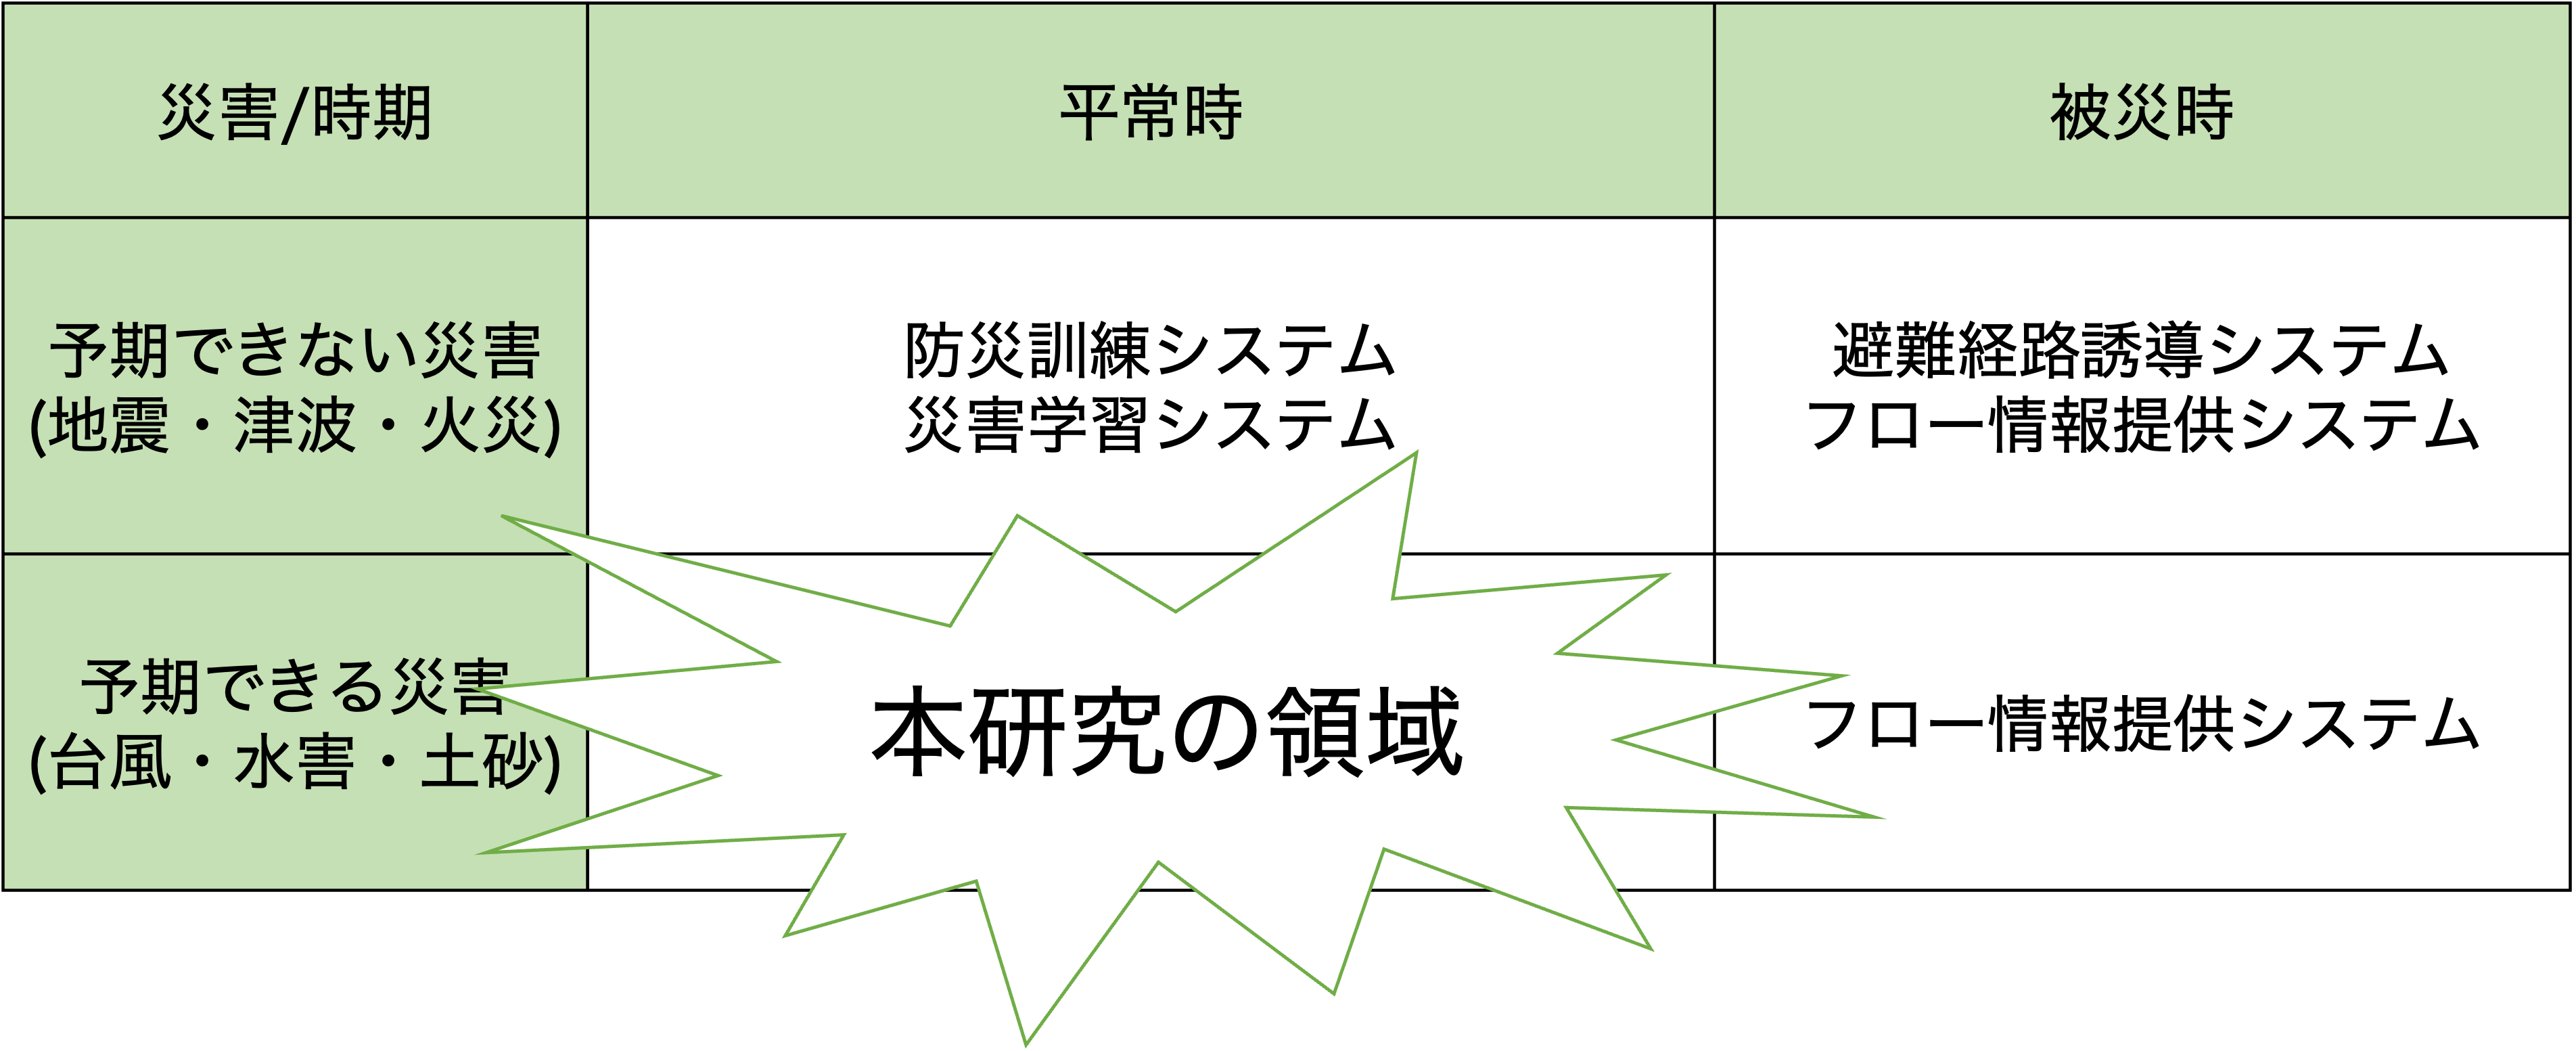
\includegraphics[height=6cm]{./fig/research_area.png}
  %\vspace{-3mm}
  \caption{研究領域の区分}
  \label{fig:reasearch_area}
  %\vspace{2mm}
\end{figure}

本研究が位置する領域は予測できる災害に対して,平常時に情報提供をする領域である.
現状災害情報システムの研究では地震に対する研究が多い.
具体的に,平常時には防災訓練を行うシステム\cite{1050574047089440256,1520577741138112640},被災時には避難経路を提示するシステムの研究がおこなわれている\cite{1050292572101475584,1050855522101622784,1050011097136129280,1390569634314138496,1390574181079225984,1050292572101463552,1520856738287330432}。
つまり,予測できる災害に対して災害情報を提供する研究領域はまだまだ未発達である.

\subsection{先行事例}
本研究の領域に関連するシステムの事例を3つ紹介する.

\subsubsection{push通知型災害情報システム}
1つ目はpush通知型の情報提供システムである.
災害が発生したときに,push通知を送ることでユーザに情報を提供するシステムである.
具体的にはSafety Tips\cite{SafetyTips}がこの種類の情報提供システムにあたる.
Safety Tipsは観光庁監修で開発された多言語災害情報提供アプリである.
国や自治体が発表する,様々な災害の情報や避難情報などのフロー情報をpush通知で知らせる.
また,ストック情報に関しての情報や緊急時の連絡先などのストック情報を提供している.

このアプリと本研究で開発したアプリの一番の違いは通知のタイミングである.
Safety Tipsでは気象庁の注意報以上のレベルの情報を用いてpush通知をするのに対して,本研究のアプリでは早期注意報を用いてpush通知をする.
本研究のアプリは通知するタイミングが早いため,訪日観光客にとって防災行動をとれる猶予を確保できる.

\subsubsection{地図ベースの情報可視化システム}
2つ目は気象情報を地図上に可視化するシステムである.
気象情報とは降水量や風速といった気象状況から予測される情報である.
具体的にはWindy\cite{Windy}がこの種類の情報提供システムにあたる.
Windyは世界中の降水量・風速などの情報を地図に可視化するアプリである.
Windy.comというチェコの企業によって開発された.
このアプリでは10日先までの降水量や風速,台風の進路の予測情報を提供している.

このアプリと本研究で開発したアプリの一番の違いは日本の地理に明るくなくても正確に情報を理解できる点である.
Windyは予測の情報を地図上に可視化して表示している.
つまり,訪日観光客は日本地図を読み取って,自身が訪れる予定の場所が災害の影響を受けるのか判断する必要がある.
本研究のアプリは訪日観光客が組み立てた旅程に基づいて,災害の影響を受けるか監視するため,訪日観光客に日本の地理に対する知識を要求しない.

\subsubsection{防災教育型情報システム}
3つ目は防災教育型の情報システムである.
志垣ら\cite{1390855511130932864}は訪日観光客に自発的に使用される防災知識提供システムを提案している.
このシステムは訪日観光客に防災知識を楽しく学習してもらうことを目的としている.
観光地に関連する防災知識を蓄えるために,イラスト付きの2択クイズを出すアプリである.

このアプリと本研究のアプリとの違いは,フロー情報を通知しない点である.
このアプリは訪日観光客が事前に能動的にアプリを使って学習する.
つまり,ストック情報について提供できるが,フロー情報について通知する機能はない.
したがって,防災行動を積極的に促すことはできない.

その他にも,Web検索途中に防災情報を提供するシステム\cite{1050292572146543616}が提案されているが,フロー情報を通知しない.

\subsection{新規性}
本研究の新規性は2点ある.
1点目は予測できる災害に対して,適切なタイミングでフロー情報とストック情報を提供する点である.
適切なタイミングとは,災害の危険性がある程度認められており,訪日観光客が防災行動をとる余裕があるタイミングである.
2点目は旅程に基づいて訪れる場所ごとに情報を提供することから,日本の地理情報を知らなくとも情報を理解できる点である.

\section{論文構成}
2章では,提案・構築したシステムについて詳説する.
3章では,システムの有用性を検証するためにおこなった実験について記述する.
最後に4章において,本研究についてまとめ,今後の課題について述べる.

\end{document}
